% ============================================================
% PHẦN 3.8 — PHỄU TIẾP CẬN VÀ CHUYỂN ĐỔI KHÁCH HÀNG
% ------------------------------------------------------------
% Thuộc: PA3-02 (phễu) + PA3-03 (hạ tầng đo lường)
% Người phụ trách chính: Nguyễn Anh Thư – CEO/Project Lead
% Phối hợp: Lê Nguyên Nhật (hạ tầng tracking)
%
% CÂU HỎI CẦN TRẢ LỜI:
%   - Khách hàng đi qua những bước chuyển đổi nào?
%   - Dữ liệu nào cần ghi lại tại từng bước?
%   - Sự kiện nào được xem là một lượt kích hoạt sản phẩm?
%   - Hệ thống sẽ ghi nhận lead, demo, pilot và người dùng trả phí ở đâu?
%
% OUTPUT BẮT BUỘC:
%   1. Phễu chuyển đổi (tối thiểu):
%      Khách hàng tiềm năng
%        → Phản hồi
%        → Đặt lịch demo
%        → Đồng ý pilot
%        → Hoàn tất onboarding
%        → Sử dụng thử
%        → Đánh giá
%        → Trả phí
%
%   2. Bảng mục tiêu cho từng tầng phễu
%      (Ghi chú: chưa cần khẳng định là kết quả thực tế)
%
%   3. Danh sách sự kiện đo lường:
%      - Truy cập landing page
%      - Nhấn xem demo
%      - Gửi biểu mẫu
%      - Đặt lịch
%      - Đồng ý pilot
%      - Hoàn thành onboarding
%      - Hoàn tất phiên thử nghiệm
%      - Chuyển sang trả phí
%
%   4. Sơ đồ luồng dữ liệu lead:
%      Từ kênh quảng bá → nơi lưu → người xử lý
%
% TIÊU CHÍ HOÀN THÀNH:
%   - Landing page phải phục vụ mục tiêu chuyển đổi, không chỉ giới thiệu sản phẩm
%   - Phải xác định nguồn dữ liệu dùng để tính KPI
% ============================================================

\subsection{Phễu tiếp cận và chuyển đổi khách hàng}

Trong phạm vi mục này, sẽ có 2 phần là chiến lược phễu và thông điệp theo từng tầng và \textbf{hạ tầng
tracking}: landing page, form thu lead, danh sách sự kiện đo lường, nơi lưu dữ
liệu và cách chuyển lead cho người xử lý. Mục tiêu là bảo đảm mọi hành động quan
trọng của khách hàng đều được ghi nhận thành dữ liệu để đánh giá hiệu quả chuyển đổi,
thay vì chỉ đánh giá chiến dịch bằng cảm tính.

\subsubsection{Khung phễu chuyển đổi cần được hệ thống ghi nhận}

Phễu chuyển đổi của 1Stream trong giai đoạn MVP được thiết kế theo mô hình B2B
có hỗ trợ trực tiếp. Khách hàng không tự mua phần mềm ngay sau khi xem quảng cáo;
họ cần đi qua các bước tìm hiểu, demo, gửi dữ liệu mẫu, chạy pilot và đánh giá
kết quả trước khi chuyển sang trả phí. Vì vậy, hệ thống cần ghi nhận tối thiểu
các trạng thái trong Bảng~\ref{tab:conversion-funnel-tracking-1stream}.

\begin{table}[H]
    \centering
    \footnotesize
    \setlength{\tabcolsep}{3pt}
    \renewcommand{\arraystretch}{1.22}
    \caption{Phễu chuyển đổi và dữ liệu cần ghi nhận ở từng tầng}
    \label{tab:conversion-funnel-tracking-1stream}
    \rowcolors{2}{paperBg}{white}
    \begin{tabularx}{\linewidth}{@{}L{2.8cm}Y Y L{2.7cm}@{}}
        \toprule
        \rowcolor{softBlue}
        \textbf{Tầng phễu} &
        \textbf{Hành động của khách hàng} &
        \textbf{Dữ liệu kỹ thuật cần ghi} &
        \textbf{Nơi lưu chính} \\ \midrule

        Khách hàng tiềm năng &
        Khách nhìn thấy nội dung, được giới thiệu hoặc được nhóm tiếp cận trực
        tiếp. &
        Nguồn kênh, tên đơn vị, ngành, khu vực, link fanpage/website, người phụ
        trách liên hệ. &
        Google Sheet/CRM lead \\

        Phản hồi &
        Khách trả lời tin nhắn, email, bình luận hoặc phản hồi qua đối tác giới
        thiệu. &
        Thời điểm phản hồi, kênh phản hồi, người phản hồi, nhu cầu ban đầu, điểm
        ICP sơ bộ. &
        CRM lead \\

        Đặt lịch demo &
        Khách đồng ý xem demo hoặc tư vấn 20--30 phút. &
        Ngày giờ demo, người tham dự, trạng thái xác nhận, link lịch, nguồn đặt
        lịch. &
        Google Calendar/CRM \\

        Đồng ý pilot &
        Khách đồng ý gửi dữ liệu mẫu hoặc chạy thử một gói giới hạn. &
        Gói pilot đề xuất, dữ liệu cần nhận, người duyệt nội dung, người duyệt
        ngân sách, trạng thái cam kết. &
        CRM pipeline \\

        Hoàn tất onboarding &
        Khách gửi đủ tài liệu và được cấu hình phiên thử nghiệm đầu tiên. &
        Checklist dữ liệu, trạng thái tài khoản/kênh live, ngày hoàn tất cấu
        hình, lỗi kỹ thuật nếu có. &
        CRM + dashboard nội bộ \\

        Sử dụng thử &
        Khách chạy phiên demo/pilot bằng video hoặc dữ liệu thật. &
        Số phiên, số giờ-kênh, trạng thái phát, số bình luận/lead được ghi nhận,
        lỗi vận hành. &
        Dashboard 1Stream/log phiên \\

        Đánh giá &
        Khách phản hồi sau pilot và quyết định có tiếp tục hay không. &
        Điểm hài lòng, vấn đề gặp phải, yêu cầu chỉnh sửa, ý định trả phí hoặc
        lý do từ chối. &
        Form khảo sát/CRM \\

        Trả phí &
        Khách ký thỏa thuận hoặc thanh toán gói đầu tiên. &
        Gói mua, giá trị hợp đồng, ngày bắt đầu, người phụ trách chăm sóc, nguồn
        chuyển đổi. &
        CRM + bảng doanh thu \\ \bottomrule
    \end{tabularx}
    \rowcolors{2}{}{}
\end{table}

Trong phễu này, một lượt \textbf{kích hoạt sản phẩm} không nên được tính ngay khi
khách chỉ gửi form. Với 1Stream, kích hoạt nên được ghi nhận khi khách hoàn tất
onboarding và có ít nhất một phiên thử nghiệm được chạy bằng dữ liệu thật hoặc
dữ liệu mẫu đã được duyệt. Đây là thời điểm khách hàng bắt đầu nhìn thấy giá trị
cốt lõi của sản phẩm: video AI, vận hành giờ-kênh và hỗ trợ thu lead.

\subsubsection{Landing page và form chuyển đổi}

Landing page của 1Stream phải đóng vai trò là điểm chuyển đổi trung tâm cho các
kênh ở mục 3.6. Trang này không chỉ giới thiệu sản phẩm, mà phải dẫn khách hàng
đến một trong ba hành động cụ thể: \textbf{đặt lịch demo}, \textbf{gửi dữ liệu
mẫu} hoặc \textbf{đăng ký pilot}. Về mặt kỹ thuật, landing page cần được thiết
kế đủ đơn giản để triển khai nhanh trong giai đoạn MVP nhưng vẫn ghi nhận được
nguồn và trạng thái của từng lead.

\begin{figure}[H]
    \centering
    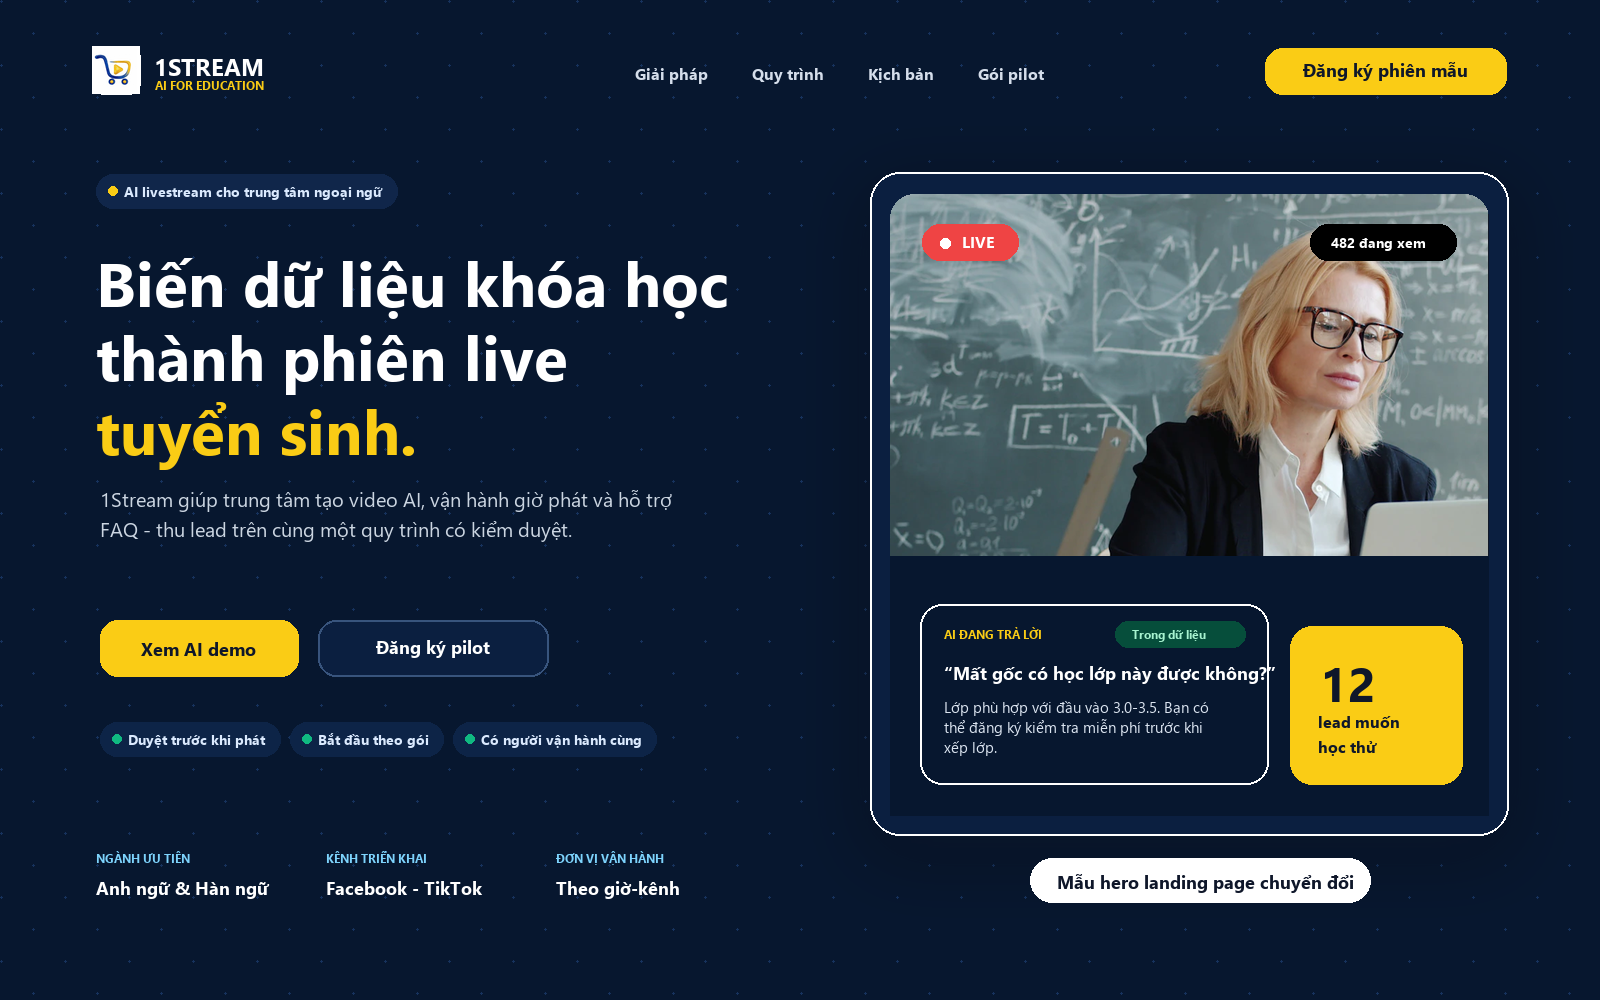
\includegraphics[width=0.95\linewidth]{imgs/PA3_pics/landing_page_hero_mockup.png}
    \caption{Mẫu giao diện hero landing page chuyển đổi của 1Stream}
    \label{fig:pa3_landing_page_hero_mockup}
\end{figure}

\begin{table}[H]
    \centering
    \small
    \setlength{\tabcolsep}{4pt}
    \renewcommand{\arraystretch}{1.22}
    \caption{Các thành phần kỹ thuật tối thiểu của landing page}
    \label{tab:landing-page-components-1stream}
    \rowcolors{2}{paperBg}{white}
    \begin{tabularx}{\linewidth}{@{}L{3.2cm}Y L{3.2cm}@{}}
        \toprule
        \rowcolor{softBlue}
        \textbf{Thành phần} & \textbf{Vai trò chuyển đổi} & \textbf{Sự kiện cần ghi} \\ \midrule

        Tiêu đề và mô tả ngắn &
        Giải thích 1Stream giúp trung tâm tạo/vận hành livestream tuyển sinh từ
        dữ liệu khóa học đã duyệt. &
        \texttt{page\_view} \\

        Video demo ngắn &
        Cho khách thấy ví dụ video AI, cách trả lời câu hỏi và cách thu lead. &
        \texttt{demo\_play}, \texttt{demo\_complete} \\

        Nút đặt lịch demo &
        Chuyển khách có nhu cầu rõ sang bước hẹn tư vấn. &
        \texttt{demo\_cta\_click}, \texttt{booking\_created} \\

        Form đăng ký pilot &
        Thu thông tin để đánh giá mức phù hợp ICP và khả năng chạy thử. &
        \texttt{form\_start}, \texttt{form\_submit} \\

        Checklist dữ liệu cần chuẩn bị &
        Giúp khách biết cần gửi học phí, lịch học, FAQ, ưu đãi và nội dung mẫu
        trước khi pilot. &
        \texttt{checklist\_download} \\

        Thông tin liên hệ Zalo/email &
        Tạo đường dự phòng cho khách chưa muốn điền form hoặc cần hỏi nhanh. &
        \texttt{contact\_click} \\ \bottomrule
    \end{tabularx}
    \rowcolors{2}{}{}
\end{table}

Form thu lead cần ngắn, nhưng đủ dữ liệu để phân biệt lead đại trà và lead phù
hợp ICP. Trong giai đoạn đầu, nhóm có thể dùng Google Form, Tally hoặc một form
đơn giản trên landing page; điều quan trọng là mỗi lượt gửi form phải tự động
đổ về một bảng dữ liệu có thể lọc, chấm điểm và phân công xử lý.

\begin{figure}[H]
    \centering
    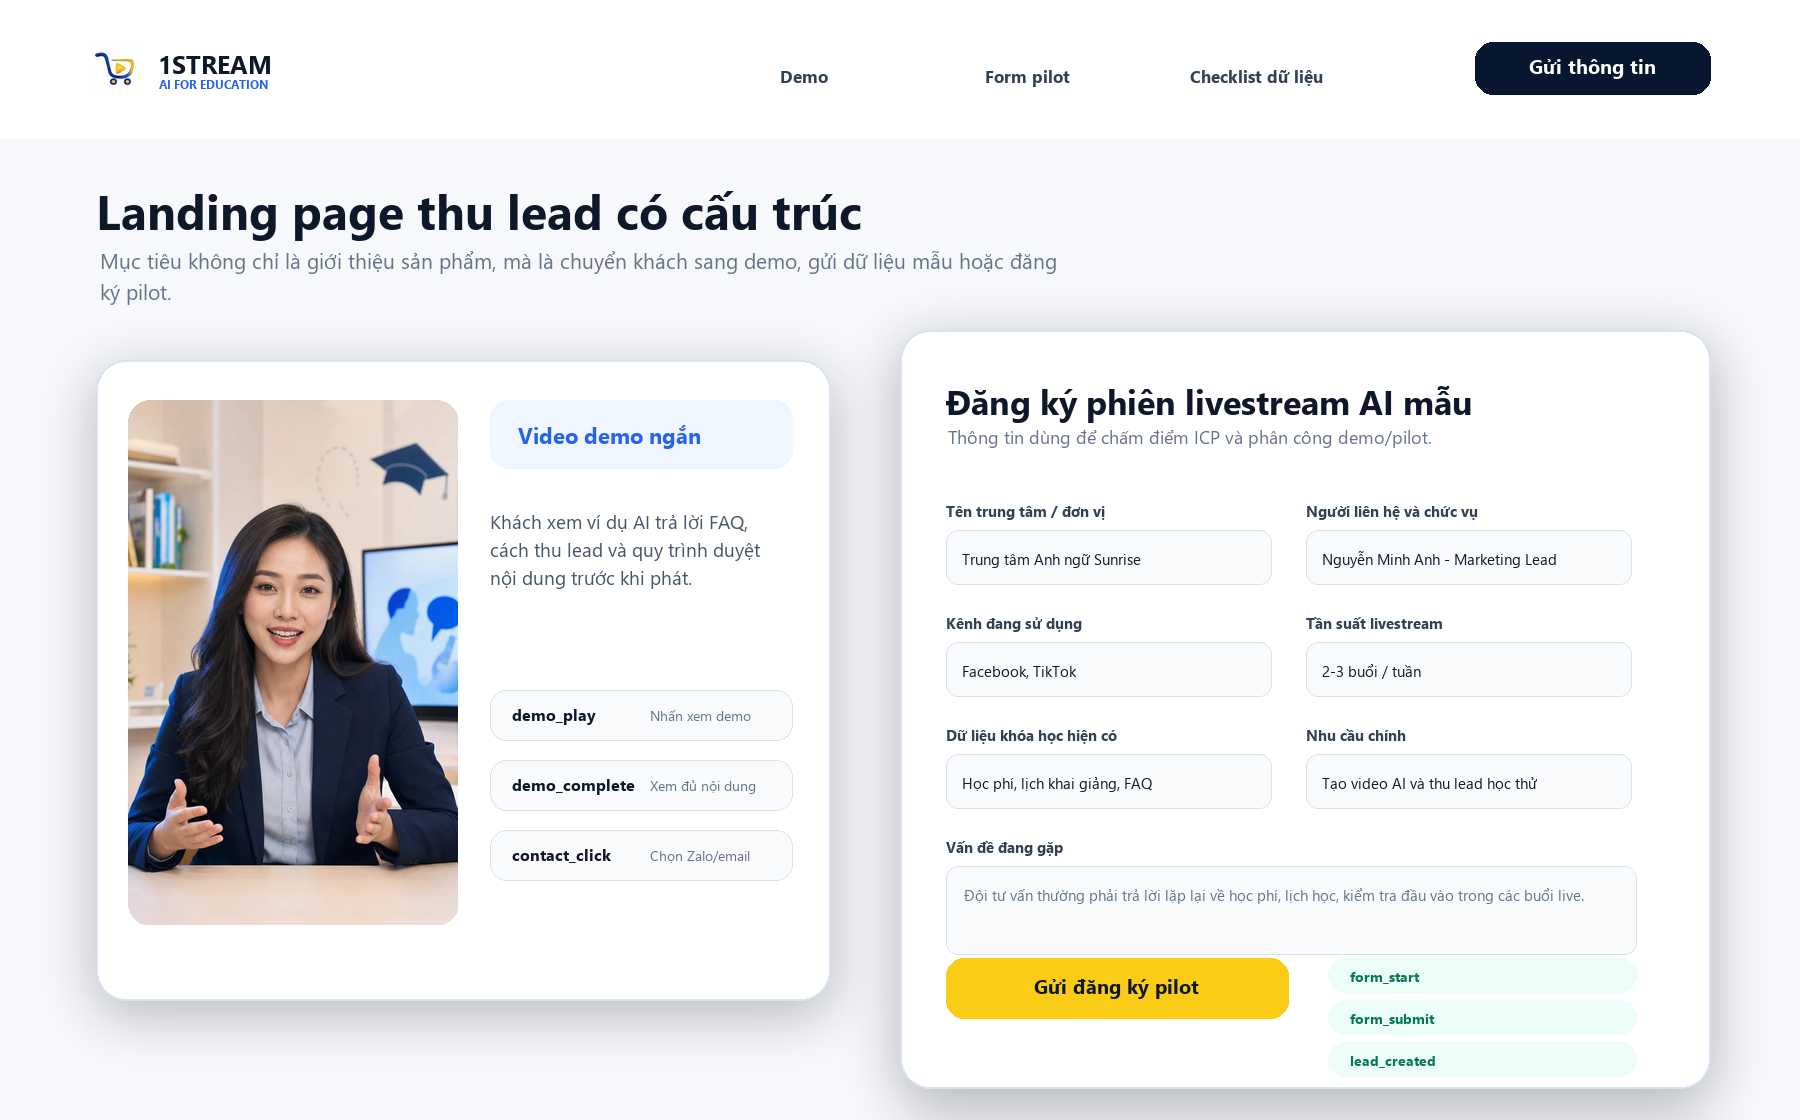
\includegraphics[width=0.95\linewidth]{imgs/PA3_pics/landing_page_form_mockup.png}
    \caption{Mẫu khu vực video demo và form đăng ký pilot trên landing page}
    \label{fig:pa3_landing_page_form_mockup}
\end{figure}

\begin{table}[H]
    \centering
    \footnotesize
    \setlength{\tabcolsep}{3pt}
    \renewcommand{\arraystretch}{1.22}
    \caption{Trường dữ liệu đề xuất trong form đăng ký demo/pilot}
    \label{tab:lead-form-fields-1stream}
    \rowcolors{2}{paperBg}{white}
    \begin{tabularx}{\linewidth}{@{}L{3.0cm}Y L{2.3cm}L{2.4cm}@{}}
        \toprule
        \rowcolor{softBlue}
        \textbf{Trường dữ liệu} &
        \textbf{Mục đích sử dụng} &
        \textbf{Bắt buộc} &
        \textbf{Dùng cho KPI} \\ \midrule

        Tên trung tâm/đơn vị &
        Nhận diện tài khoản khách hàng và tránh trùng lead. &
        Có &
        Lead, ICP \\

        Ngành đào tạo/dịch vụ &
        Kiểm tra có thuộc trung tâm ngoại ngữ hoặc đơn vị bán khóa học hay không. &
        Có &
        Lead phù hợp ICP \\

        Khu vực hoạt động &
        Ưu tiên TP.HCM hoặc khu vực nhóm có thể hỗ trợ trực tiếp. &
        Có &
        ICP, SOM \\

        Người liên hệ và chức vụ &
        Phân biệt chủ trung tâm, trưởng marketing, tư vấn tuyển sinh hoặc nhân
        sự vận hành. &
        Có &
        SQL \\

        Số điện thoại/email/Zalo &
        Dùng để xác nhận demo, chăm sóc sau form và chuyển lead cho người xử lý. &
        Có &
        Tỷ lệ phản hồi \\

        Kênh đang sử dụng &
        Biết khách đang hoạt động trên Facebook, TikTok, YouTube hoặc kênh khác. &
        Có &
        Sẵn sàng kênh \\

        Tần suất livestream &
        Đánh giá cường độ vấn đề và khả năng dùng gói giờ-kênh. &
        Có &
        Lead phù hợp ICP \\

        Dữ liệu khóa học hiện có &
        Xác định khách đã có học phí, lịch học, FAQ, ưu đãi và tài liệu để
        onboarding hay chưa. &
        Có &
        Onboarding \\

        Nhu cầu chính &
        Phân loại khách cần tạo video, vận hành giờ phát, thu lead hoặc gói trọn
        bộ. &
        Có &
        Demo/pilot \\

        Ghi chú hoặc vấn đề đang gặp &
        Thu insight định tính cho sales và product. &
        Không &
        Phản hồi khách hàng \\ \bottomrule
    \end{tabularx}
    \rowcolors{2}{}{}
\end{table}

\subsubsection{Danh sách sự kiện tracking}


\begin{table}[H]
    \centering
    \footnotesize
    \setlength{\tabcolsep}{3pt}
    \renewcommand{\arraystretch}{1.18}
    \caption{Danh sách sự kiện tracking đề xuất cho phễu 1Stream}
    \label{tab:tracking-events-1stream}
    \rowcolors{2}{paperBg}{white}
    \begin{tabularx}{\linewidth}{@{}L{3.2cm}Y Y L{2.4cm}@{}}
        \toprule
        \rowcolor{softBlue}
        \textbf{Event name} &
        \textbf{Khi nào ghi nhận} &
        \textbf{Thông tin đi kèm} &
        \textbf{Nguồn dữ liệu} \\ \midrule

        \texttt{lead\_created} &
        Khi một khách hàng được thêm vào danh sách từ outreach, cộng đồng, đối
        tác hoặc form. &
        Nguồn kênh, tên đơn vị, ngành, khu vực, người phụ trách. &
        CRM/Sheet \\

        \texttt{page\_view} &
        Khi khách truy cập landing page. &
        UTM source, UTM campaign, thiết bị, thời điểm truy cập. &
        Web analytics \\

        \texttt{demo\_play} &
        Khi khách nhấn xem video demo. &
        Vị trí video, nguồn truy cập, thời lượng xem nếu đo được. &
        Web analytics \\

        \texttt{form\_submit} &
        Khi khách gửi form đăng ký demo hoặc pilot. &
        Toàn bộ trường form, nguồn kênh, thời điểm gửi. &
        Form/CRM \\

        \texttt{booking\_created} &
        Khi khách đặt lịch demo thành công. &
        Ngày giờ demo, người phụ trách, trạng thái xác nhận. &
        Calendar/CRM \\

        \texttt{demo\_completed} &
        Khi buổi demo đã diễn ra. &
        Người tham dự, nhu cầu, phản đối chính, mức phù hợp ICP. &
        CRM \\

        \texttt{pilot\_agreed} &
        Khi khách đồng ý chạy thử hoặc gửi dữ liệu mẫu. &
        Gói pilot, phạm vi thử nghiệm, người duyệt nội dung, deadline dữ liệu. &
        CRM \\

        \texttt{onboarding\_completed} &
        Khi khách gửi đủ dữ liệu và nhóm cấu hình xong phiên thử nghiệm. &
        Trạng thái dữ liệu, kênh live, tài khoản, lỗi còn tồn tại. &
        Dashboard/CRM \\

        \texttt{trial\_session\_completed} &
        Khi phiên thử nghiệm đầu tiên hoàn tất. &
        Số giờ-kênh, số bình luận, số lead ghi nhận, trạng thái phát. &
        Dashboard/log phiên \\

        \texttt{feedback\_submitted} &
        Khi khách gửi đánh giá sau demo hoặc sau pilot. &
        Điểm hài lòng, vấn đề, ý định tiếp tục, yêu cầu chỉnh sửa. &
        Survey/CRM \\

        \texttt{paid\_conversion} &
        Khi khách ký hợp đồng hoặc thanh toán gói đầu tiên. &
        Gói mua, giá trị, ngày bắt đầu, nguồn lead, người phụ trách. &
        CRM/bảng doanh thu \\ \bottomrule
    \end{tabularx}
    \rowcolors{2}{}{}
\end{table}

Trong giai đoạn chưa có hệ thống analytics hoàn chỉnh, 1Stream không cần xây
dashboard phức tạp ngay. Nhóm có thể bắt đầu bằng một Google Sheet hoặc Airtable
với các cột cố định, sau đó nhập liệu bán tự động từ form và cập nhật thủ công
các sự kiện như demo, pilot, onboarding hoặc trả phí. Khi số lượng lead tăng,
cấu trúc này có thể được chuyển sang CRM hoặc dashboard nội bộ mà không phải đổi
lại định nghĩa KPI.

\subsubsection{Luồng dữ liệu lead và phân công xử lý}

Luồng dữ liệu lead cần đủ rõ để trả lời câu hỏi: lead đến từ đâu, được lưu ở đâu,
ai chịu trách nhiệm và trạng thái hiện tại là gì. Đối với MVP, luồng dữ liệu đề
xuất như sau:

\begin{center}
\small
\textbf{Kênh quảng bá} $\rightarrow$
\textbf{Landing page / Inbox / Đối tác} $\rightarrow$
\textbf{Form hoặc CRM lead} $\rightarrow$
\textbf{Chấm điểm ICP} $\rightarrow$
\textbf{Người phụ trách demo/pilot} $\rightarrow$
\textbf{Dashboard hoặc báo cáo sau pilot}
\end{center}

\begin{figure}[H]
    \centering
    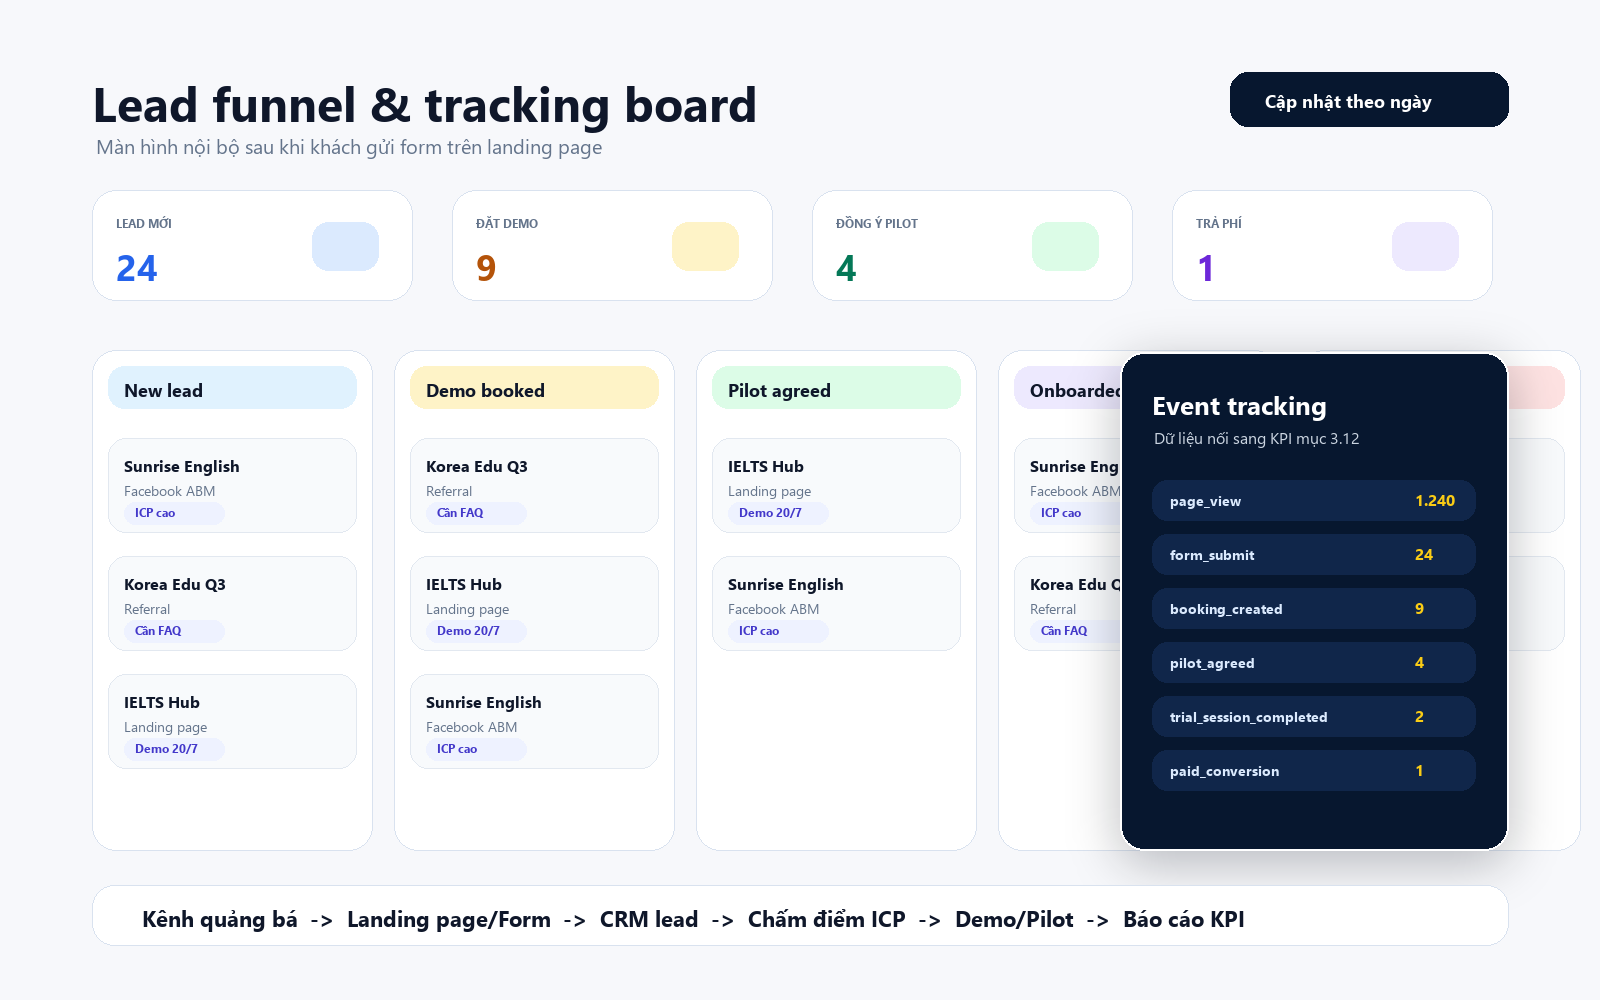
\includegraphics[width=0.95\linewidth]{imgs/PA3_pics/landing_page_tracking_mockup.png}
    \caption{Mẫu bảng theo dõi lead và sự kiện tracking sau khi khách gửi form}
    \label{fig:pa3_landing_page_tracking_mockup}
\end{figure}

\begin{table}[H]
    \centering
    \small
    \setlength{\tabcolsep}{4pt}
    \renewcommand{\arraystretch}{1.22}
    \caption{Nơi lưu dữ liệu và người xử lý theo từng loại lead}
    \label{tab:lead-data-flow-ownership-1stream}
    \rowcolors{2}{paperBg}{white}
    \begin{tabularx}{\linewidth}{@{}L{3.1cm}Y L{3.0cm}L{2.5cm}@{}}
        \toprule
        \rowcolor{softBlue}
        \textbf{Nguồn lead} & \textbf{Cách ghi nhận} & \textbf{Người xử lý chính} & \textbf{Trạng thái cần cập nhật} \\ \midrule

        Tiếp cận trực tiếp/ABM &
        Nhập vào CRM/Sheet ngay khi thêm tài khoản mục tiêu; cập nhật sau mỗi
        lần nhắn tin/gọi điện. &
        Quang + Nhật  &
        New, Contacted, Replied \\

        Landing page/form &
        Tự động ghi vào Sheet/CRM khi khách gửi form; giữ lại UTM/source nếu có. &
        Quang &
        Submitted, Qualified, Demo booked \\

        Workshop/webinar &
        Danh sách đăng ký và danh sách tham dự được nhập vào CRM; gắn tag theo
        tên sự kiện. &
        Quang + Thư&
        Registered, Attended, Follow-up \\

        Đối tác giới thiệu &
        Tạo lead mới kèm tên đối tác giới thiệu và mức độ tin cậy ban đầu. &
        Thư &
        Referral, Demo booked, Pilot proposed \\

        Pilot/sử dụng thử &
        Dữ liệu vận hành lấy từ dashboard hoặc log phiên; kết quả tổng hợp lại
        vào CRM. &
        Nhật + Cảnh &
        Onboarded, Trial completed, Feedback collected \\

        Khách trả phí &
        Ghi nhận gói mua, giá trị, ngày bắt đầu và nguồn lead ban đầu. &
        Toàn + Thư&
        Paid, Retained, Upsell candidate \\ \bottomrule
    \end{tabularx}
    \rowcolors{2}{}{}
\end{table}

Về trách nhiệm kỹ thuật, cần bảo đảm ba điều kiện tối thiểu. Thứ nhất, mọi
lead đều có \textbf{nguồn kênh} để sau này tính hiệu quả từng kênh. Thứ hai, mọi
lead đều có \textbf{trạng thái phễu} để biết đang ở bước nào và ai cần xử lý.
Thứ ba, các sự kiện quan trọng như đặt lịch demo, đồng ý pilot, hoàn tất
onboarding và hoàn tất phiên thử nghiệm phải có \textbf{ngày giờ ghi nhận}, vì
đây là dữ liệu dùng để tính tốc độ chuyển đổi và thời gian từ đăng ký đến phiên
đầu tiên.

\subsubsection{Bảng dữ liệu đo lường cho phễu chuyển đổi}

Các sự kiện tracking cần được định nghĩa thống nhất để nhóm có thể đọc kết quả
phễu theo cùng một cách. Nếu không xác định trước sự kiện và nguồn dữ liệu, các
chỉ số như tỷ lệ đặt lịch demo, tỷ lệ hoàn thành onboarding hoặc CAC sẽ khó tính
nhất quán. Bảng dưới đây tóm tắt dữ liệu cần thu và ý nghĩa của từng nhóm chỉ số.

\begin{table}[H]
    \centering
    \small
    \setlength{\tabcolsep}{4pt}
    \renewcommand{\arraystretch}{1.2}
    \caption{Sự kiện tracking và nhóm chỉ số cần đo trong phễu chuyển đổi}
    \label{tab:tracking-to-kpi-1stream}
    \rowcolors{2}{paperBg}{white}
    \begin{tabularx}{\linewidth}{@{}L{3.4cm}Y Y@{}}
        \toprule
        \rowcolor{softBlue}
        \textbf{Nhóm chỉ số cần đo} & \textbf{Sự kiện/nguồn dữ liệu sử dụng} & \textbf{Ý nghĩa đối với quyết định kênh} \\ \midrule

        Số người tiếp cận &
        \texttt{page\_view}, analytics từ Facebook/TikTok/LinkedIn, danh sách
        outreach. &
        Biết kênh nào tạo được độ phủ ban đầu. \\

        Lượt đăng ký dùng thử/demo &
        \texttt{form\_submit}, \texttt{booking\_created}. &
        Biết kênh nào tạo nhu cầu thật, không chỉ lượt xem. \\

        Tỷ lệ phản hồi từ tiếp cận trực tiếp &
        Số lead trạng thái Replied chia cho số lead Contacted. &
        Đánh giá chất lượng danh sách ABM và thông điệp outreach. \\

        Tỷ lệ demo sang pilot &
        \texttt{demo\_completed}, \texttt{pilot\_agreed}. &
        Biết demo có đủ thuyết phục và khách có đủ điều kiện thử nghiệm không. \\

        Tỷ lệ hoàn thành onboarding &
        \texttt{pilot\_agreed}, \texttt{onboarding\_completed}. &
        Kiểm tra khách có dữ liệu đủ chuẩn và quy trình setup có quá khó không. \\

        Thời gian từ đăng ký đến phiên đầu tiên &
        Thời điểm \texttt{form\_submit} đến \texttt{trial\_session\_completed}. &
        Đánh giá tốc độ triển khai của quy trình kỹ thuật. \\

        Số lead ghi nhận trong pilot &
        Log phiên live, dashboard bình luận/lead, báo cáo sau pilot. &
        Chứng minh giá trị vận hành của 1Stream trong tình huống thật. \\

        Phản hồi và mức hài lòng &
        \texttt{feedback\_submitted}, form khảo sát sau pilot. &
        Xác định điểm cần cải thiện và khả năng chuyển sang trả phí. \\

        Khách hàng trả phí mới &
        \texttt{paid\_conversion}, CRM/bảng doanh thu. &
        Là dữ liệu đầu ra để tính CAC và hiệu quả thương mại. \\ \bottomrule
    \end{tabularx}
    \rowcolors{2}{}{}
\end{table}

Tóm lại, landing page và form giúp thu lead có cấu trúc; danh sách sự kiện giúp
ghi nhận hành vi theo từng bước; CRM/Sheet giúp đội ngũ biết ai đang xử lý lead;
dashboard/log phiên giúp chứng minh giá trị trong pilot. Khi các dữ liệu này
được ghi nhận đều đặn, nhóm có thể đánh giá khách quan kênh nào nên tiếp tục,
kênh nào cần điều chỉnh và kênh nào nên tạm dừng.
